%
% chap006.tex
%

\chapter{Summe der ersten $n$ Quadratzahlen von natürlichen Zahlen}

Abu Ali al-Hasan Ibn al-Haitham (965-1039), der im Deutschen unter
Alhazen und im Arabischen unter Ibn al-Haitham bekannt ist,
war ein bedeutender arabischer Mathematiker und Physiker.
Besondere wissenschaftliche Beiträge brachte er auf dem Gebiet
der Optik und der experimentellen Methodik.
Für seine Experimente auf diesem Gebiet gab man ihn den Beinamen
``Vater der Optik''. Es gilt als der Erfinder der Lupe und
damit der Mikroskopie. Die Formel zur Bestimmung der Summe der ersten
$n$ Quadratzahlen von natürlichen Zahlen wurde ebenfalls von
ihm entdeckt.

\begin{figure}[H]
  \centering
  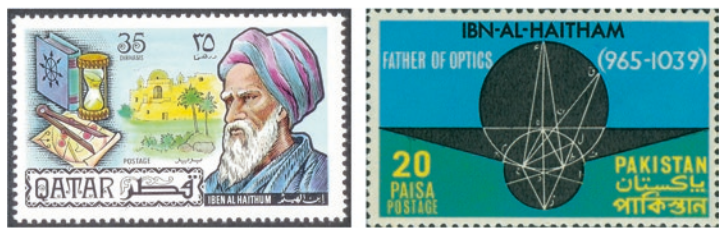
\includegraphics[width=.5\linewidth]{./images/muster06.png}
  \caption[]{Mathematiker und Physiker Abu Ali al-Hasan ibn al-Haitham (965-1039).}
  \label{fig:abu_ali_al_Hasan_ahitham}
\end{figure}


